\documentclass{article}
\usepackage{tikz,amsmath}
\usetikzlibrary{shapes.geometric, arrows}
\usepackage[paperheight=6.5in,paperwidth=4.8in,margin=0.1in]{geometry}

\tikzstyle{process} = [rectangle, minimum width=3em, minimum height=2em, text centered, draw=blue, fill=gray!10]
\tikzstyle{startend} = [ellipse, minimum width=2em, minimum height=1em, text centered, draw=red, fill=gray!10]
\tikzstyle{arrow} = [thick,->,>=stealth]
\pagestyle{plain}

\begin{document}
\begin{figure}
\centering
\hfill\\
{\scriptsize 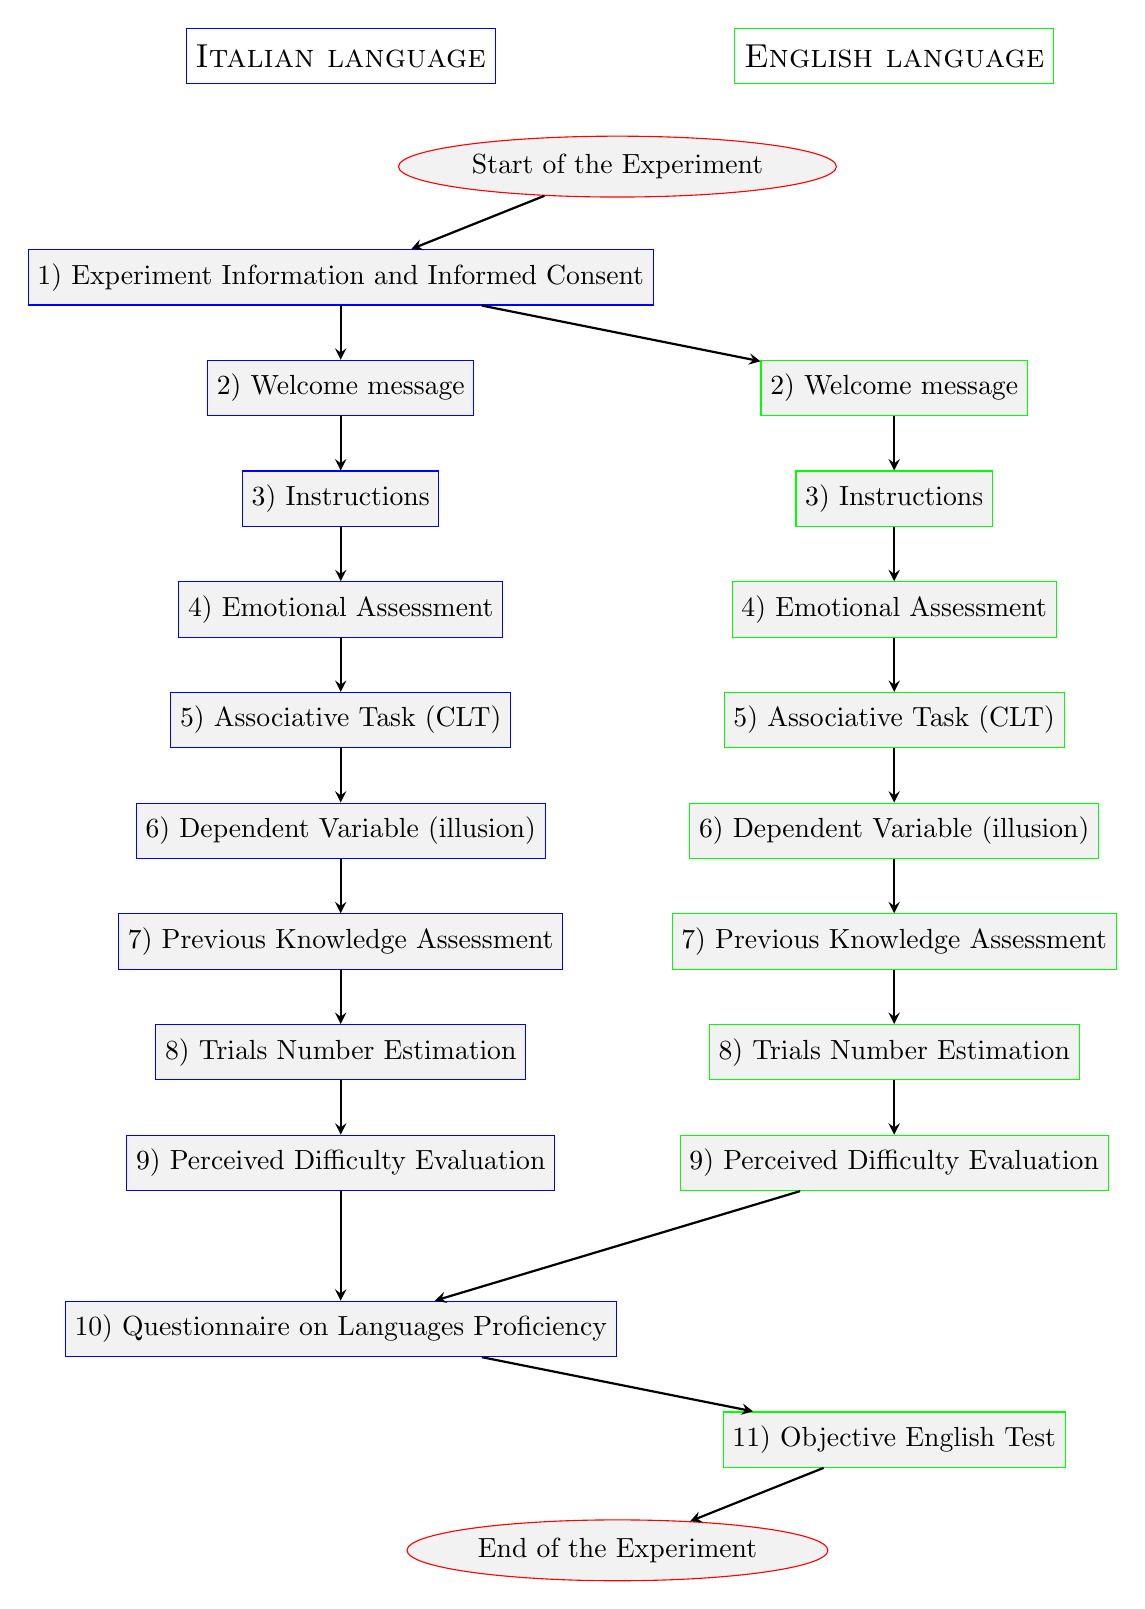
\begin{tikzpicture}[node distance=2em]

% Start 
\node (F2) [process,  yshift=-2em, xshift=-10em, fill=white] {\textsc{\large Italian language}};
\node (F3) [process,  yshift=-2em, xshift=10em, draw=green, fill=white] {\textsc{\large English language}}; 

\node (S) [startend, below of=F2, yshift=-2em, xshift=10em,] {Start of the Experiment};

% Italian side (Shifted to the left)
\node (S1) [process, below of=S, yshift= -2em, xshift=-10em] {1) Experiment Information and Informed Consent};
\node (S2) [process, below of=S1, yshift=-2em] {2) Welcome message};
\node (S3) [process, below of=S2, yshift=-2em] {3) Instructions};
\node (S4) [process, below of=S3, yshift=-2em] {4) Emotional Assessment};
\node (S5) [process, below of=S4, yshift=-2em] {5) Associative Task (CLT)};
\node (S6) [process, below of=S5, yshift=-2em] {6) Dependent Variable (illusion)};
\node (S7) [process, below of=S6, yshift=-2em] {7) Previous Knowledge Assessment};
\node (S8) [process, below of=S7, yshift=-2em] {8) Trials Number Estimation};
\node (S9) [process, below of=S8, yshift=-2em] {9) Perceived Difficulty Evaluation};

% English side (Shifted to the right)
\node (S34b) [process, below of=S1, yshift=-2em, xshift=20em,  draw=green] {2) Welcome message};
\node (S35) [process, below of=S34b, yshift=-2em, draw=green] {3) Instructions};
\node (S36) [process, below of=S35, yshift=-2em, draw=green] {4) Emotional Assessment};
\node (S37) [process, below of=S36, yshift=-2em, draw=green] {5) Associative Task (CLT)};
\node (S38) [process, below of=S37, yshift=-2em, draw=green] {6) Dependent Variable (illusion)};
\node (S39) [process, below of=S38, yshift=-2em, draw=green] {7) Previous Knowledge Assessment};
\node (S40) [process, below of=S39, yshift=-2em, draw=green] {8) Trials Number Estimation};
\node (S41) [process, below of=S40, yshift=-2em, draw=green] {9) Perceived Difficulty Evaluation};

% Linguistic Questionnaire and English Test
\node (Qe) [process, below of=S9, yshift=-4em] {10) Questionnaire on Languages Proficiency};

\node (Pe) [process, below of=Qe, yshift=-2em, xshift=20em, draw=green]{11) Objective English Test};
\node (F) [startend, below of=Pe, yshift=-2em, xshift=-10em] {End of the Experiment};

% Connecting arrows
\draw [arrow] (S) -- (S1);
\draw [arrow] (S1) -- (S2);
\draw [arrow] (S2) -- (S3);
\draw [arrow] (S3) -- (S4);
\draw [arrow] (S4) -- (S5);
\draw [arrow] (S5) -- (S6);
\draw [arrow] (S6) -- (S7);
\draw [arrow] (S7) -- (S8);
\draw [arrow] (S8) -- (S9);

\draw [arrow] (S1) -- (S34b);
\draw [arrow] (S34b) -- (S35);
\draw [arrow] (S35) -- (S36);
\draw [arrow] (S36) -- (S37);
\draw [arrow] (S37) -- (S38);
\draw [arrow] (S38) -- (S39);
\draw [arrow] (S39) -- (S40);
\draw [arrow] (S40) -- (S41);

\draw [arrow] (S9) -- (Qe);
\draw [arrow] (S41) -- (Qe);
\draw [arrow] (Qe) -- (Pe);
\draw [arrow] (Pe) -- (F);

\end{tikzpicture}}
\end{figure}
\end{document}
